\section{Aspetti implementativi}



\subsection{Il desing pattern MVC}
Il sistema e' stato implementato utilizzando il design pattern \textbf{MVC},
Model View Controller, questo design pattern aiuta lo sviluppo di applicazioni
``a camere stagne", separando il modello (la logica e il motore di gioco) dalla
grafica e dalla sua presentazione all'utente tramite un'entita' denominata
\textbf{controller}, nello scenario del progetto questa entita' e' stata
dotata della logica di gestione distribuita dello stato dei vari mondi di gioco.

\subsection{Implementazione dello schema di gioco}


In questo paragrafo vedremo brevemente l'implementazione dello schema e
della logica di gioco.
La figura \ref{img:model} mostra il diagramma delle classi del
componente model il quale racchiude tutte le funzionalità della logica
di gioco.\\
Nello specifico il model contiene tutte le funzionalità che permettono
il collegamento logico delle tessere fra di loro. 
Inoltre la logica, come anticipato dalla fase progettuale, implementa i meccanismi per rilevare il completamento degli elementi
(città, strade, monasteri) ed assegnare i punti ai loro rispettivi
proprietari.
\begin{figure}
\includegraphics[width=\textwidth]{img/modelClassDiagram.png}
\caption{Diagramma delle classi del modello di gioco}
\label{img:model}
\end{figure}

\subsection{L'interfaccia grafica}
L'interfaccia grafica e` basata sul motore Slick2D\ref{}, %TODO [citation needed]  
questo mette a disposizione una libreria abbastanza semplice per realizzare interfacce grafice
anche complesse prive di rendering 3D.

L'intera esecuzione dell'inferfaccia grafica e` affidata ad un thread dedicato, una
classe principale gestisce il dispatching degli aggiornamenti grafici e la lettura
dell'input.

Il motore di gioco lancia la funzione di rendering alla frequenza impostata, la classe principale
delega dunque la composizione della schermata alla scena attualmente caricata.
In parallelo viene anche lanciata (con cadenza meno regolare) una funzione di aggiornamento (\texttt{void update()}) che interroga il controller e recupera nel thread della grafica gli aggiornamenti pendenti, se ce ne sono (ad esempio tessere piazzate e punteggi segnati).

Alla stessa maniera, la gestione degli input viene passata alla scena corrente dalla classe principale in modo da interpretare le pressioni dei tasti e i movimenti del mouse nella maniera corretta.

\subsubsection{Interazione}
\begin{figure}[htbp]
	\includegraphics[width=\textwidth]{img/effects.jpg}
	\caption{Schermata di gioco}
	\label{img:game}
\end{figure}

In figura \ref{img:game} e` mostrata una schermata di gioco, la parte centrale e` occupata dal tavolo su cui vengono piazzate le tessere ed i meeple. 
Sui contorni della visuale di gioco vengono mostrati gli elementi dell'HUD (\emph{Heads-Up Display}): 
\begin{itemize}
\item in alto a sinistra i punteggi attuali dei partecipanti ancora in gioco;
\item in alto a destra compare un pulsante per attivare e disattivare lo zoom quando lo scenario eccede i limiti dell'HUD stesso, in questo caso si puo` spostare la visuale muovendo il puntatore verso i bordi della schermata oppure utilizando le frecce direzionali sulla tastiera;
\item in basso a sinistra i meeple ancora in mano al giocatore.
\end{itemize}
Inoltre se un giocatore e` di turno l'HUD conterra` anche:
\begin{itemize}
\item in basso al centro il pulsante di confema del piazzamento;
\item in basso a destra la tessera da piazzare;
\item \emph{una volta confermato il piazzamento} (fig. \ref{img:gameMeeple}) sulla tessera da piazzare vengono evidenziate le posizioni su cui e` possibile mettere un meeple (ammesso che il giocatore ne abbia ancora in mano).
\end{itemize}

Il giocatore di turno, spostando il mouse sui confini dello scenario creato, puo vedere un contorno nero che indica la possibilita` di tentare un piazzamento. Un click sinistro del mouse effettuera` il tentativo, mostrando la tessera in trasparenza se il piazzamento e` possibile o un effetto rosso in caso contrario. 
Utilizzando la rotellina del mouse o il click destro e` possibile ruotare la tessera.

\begin{figure}[htbp]
	\includegraphics[width=\textwidth]{img/meeplePlacement.jpg}
	\caption{Schermata di gioco: piazzamento meeple}
	\label{img:gameMeeple}
\end{figure}

Una volta confermato il piazzamento si puo` decidere di mettere un meeple su un elemento della tessera appena piazzata cliccando sul contorno del meeple e lo si puo` rimuovere cliccando sul meeple stesso.

Al termine di un turno ogni giocatore vedra` i risultati del piazzamento effettuato, gli elementi del territorio completati vengono evidenziati e, se qualche giocatore li possedeva, il punteggio dei singoli elementi viene mostratoagli stessi, come anche il piazzamento o la restituzione dei meeple.

\subsection{La gestione e la distribuzione della rete}
	\subsubsection{Registrazione presso la lobby}
		Il primo passo svolto da ogni nodo di rete e' la registrazione
		presso un server centralizzato comune, che implementa una o piu'
		``stanze" di gioco; le cosiddette lobby.\\
		Questo server aspetta la registrazione del numero
		specificato di partecipanti, inviando loro la lista dei
		giocatori per poi lasciargli il pieno controllo, chiudendo la stanza.

% TODO struttura pacchetti???
\begin{figure}[H]
\begin{minipage}[t]{0.45\textwidth}
\centering
\begin{tikzpicture}[->,
	main node/.style={circle,draw,thick,fill=green!20,minimum size=4mm},
	lobby node/.style={ellipse,draw,thick,fill=blue!20,minimum size=4mm}
]
	\node[lobby node] (L) {Lobby Server};

	\node[main node, below of=L,xshift=-18mm,yshift=-5mm] (1) {1};
	\node[main node, below of=L,xshift=-7mm,yshift=-10mm] (2) {2};
	\node[main node, below of=L,xshift=7mm, yshift=-10mm] (3) {3};
	\node[main node, below of=L,xshift=18mm,yshift=-5mm] (4) {4};

	\draw[->] (1) to[bend left=10] (L);
	\draw[->] (L) to[bend left=10] (1);

	\draw[->] (2) to[bend left=10] (L);
	\draw[->] (L) to[bend left=10] (2);

	\draw[->] (3) to[bend left=10] (L);
	\draw[->] (L) to[bend left=10] (3);

	\draw[->] (4) to[bend left=10] (L);
	\draw[->] (L) to[bend left=10] (4);
\end{tikzpicture}
\caption{\scriptsize Registrazione presso il server lobby}
\end{minipage}
\begin{minipage}[t]{0.45\textwidth}
\centering
\begin{tikzpicture}[->,
	main node/.style={circle,draw,thick,fill=green!20,minimum size=4mm},
	notacc node/.style={circle,draw,thick,fill=red!20,minimum size=4mm},
	lobby node/.style={ellipse,draw,thick,fill=blue!20,minimum size=4mm}
]
	\node[lobby node] (L) {Lobby Server};

	\node[main node, below of=L,xshift=-18mm,yshift=-5mm] (1) {1};
	\node[main node, below of=L,xshift=-7mm,yshift=-10mm] (2) {2};
	\node[main node, below of=L,xshift=7mm, yshift=-10mm] (3) {3};
	\node[main node, below of=L,xshift=18mm,yshift=-5mm] (4) {4};

	\node[notacc node,below of=L,yshift=-18mm] (5) {5};

	\draw[->] (5) to[bend left=10] (L);
	\draw[->] (L) to[bend left=10] (5);

\end{tikzpicture}
\caption{\scriptsize Eccezione del server alla richiesta di una lobby chiusa}
\end{minipage}
\end{figure}

\subsubsection{Lo schema con leader dinamico.}
Lo schema di distribuzione si basa sull'elezione di un leader "dinamico", questo
leader e' deciso in base ad un lancio di un dado iniziale (nella realta'
implementato come un random intero a 32 bit, per evitare lanci ripetuti). Il
lancio viene distribuito tra i vari player, 
il giocatore con punteggio maggiore viene
dichiarato come leader corrente, e da li a decrescere.
Inoltre il valore del tiro di dado del leader iniziale viene utilizzato da tutti i giocatori come seme per mescolare il mazzo di tessere, in modo da mantenere lo stato inizale coerente.\\
La topologia risulta quindi una rete monodirezionale con passaggio del
testimone (token ring) per la decisione del leader corrente.


\subsubsection{Aggiornamenti allo stato}
	Uno degli aspetti piu' importanti del sistema di comunicazione del gioco
	e' la presenza di classi di differenza (classe \textbf{TurnDiff}), le
	suddette classi rendono la comunicazione il piu' leggero possibile
	essendo composte da:\\

\begin{minipage}{.60\textwidth}
	\begin{itemize}
		\item Le coordinate della tessera;
		\item la rotazione della tessera posizionata;
		\item le posizioni relative del meeple se presente;
		\item il turno e il giocatore correnti.
	\end{itemize}
\end{minipage}
\begin{minipage}{.20\textwidth}
	\includegraphics{img/turndiff.png}
\end{minipage}

\subsubsection{Tolleranza ai guasti}
	Il sistema risulta tollerante ai guasti di tipo crash.
	Nel caso di un guasto di tipo crash sul nodo leader corrente, sara' il
	sistema ad invocare un'eccezione di tipo \textbf{RemoteException} verso
	i nodi interroganti, che lo elimineranno quindi dalla loro lista di
	interrogazione, riconfigurando l'anello.\\
	Nel caso di un guasto di un nodo intermedio il risultato sara' il
	medesimo al momento di un'interrogazione da parte dei vari nodi
	dell'anello (e.g. quando il nodo crashato sara` di turno).\\
	Questo genere di configurazione mantiene coerente lo stato locale delle
	diverse istanze, poiche' ogni nodo aspetta la risoluzione delle varie
	mosse ad esso precedenti prima di essere interrogato a sua volta e poter
	agire.\\
	Questo schema e' banalmente possibile utilizzando una semplice rete di
	tipo token ring, ma e' stato scelto di implementare il tutto come una
	sorta di cricca per l'aggiornamento automatico e la visualizzazione dei
	risultati con latenze brevi: se si fosse ponderato per una struttura
	completamente circolare (utilizzante lo stesso modello logico) gli
	aggiornamenti allo stato locale sarebbero applicati solamente dopo che
	il controllo (e quindi la leadership) fosse tornata al nodo richiedente,
	risultando in un'attesa pari ad \textbf{N-1} turni; essendo il gioco
	in questione un gioco di logica non propriamente reattivo e con turni
	di gioco potenzialmente molto lunghi e riflessivi, abbiamo optato
	per un modello piu' pesante da un punto di vista
	di scambio di informazioni, ma, allo stesso tempo, piu` reattivo per tutti i client,
	che comunque non e` pesante per la rete.

	Le informazioni aggiuntive di numero di turno (clock logico) e nome del giocatore presenti nel diff vengono utilizzate insieme ad un id di gioco stabilito ad inizio partita per identificare guasti arbitrari: tutte le richeste verso il giocatore di turno specificano il clock e l'id della partita e vengono controllate da quest'ultimo prima di restituire il diff, allo stesso modo il diff deve contenere il nome del player che ha appena giocato e il clock logico del suo turno.
	Questo doppio controllo consente ai nodi di verificare con sufficiente confidenza che le informazioni conenute nel diff non siano frutto di un malfunzionamento e che i nodi richiedenti siano ancora sani.

\begin{figure}[H]
	\centering
	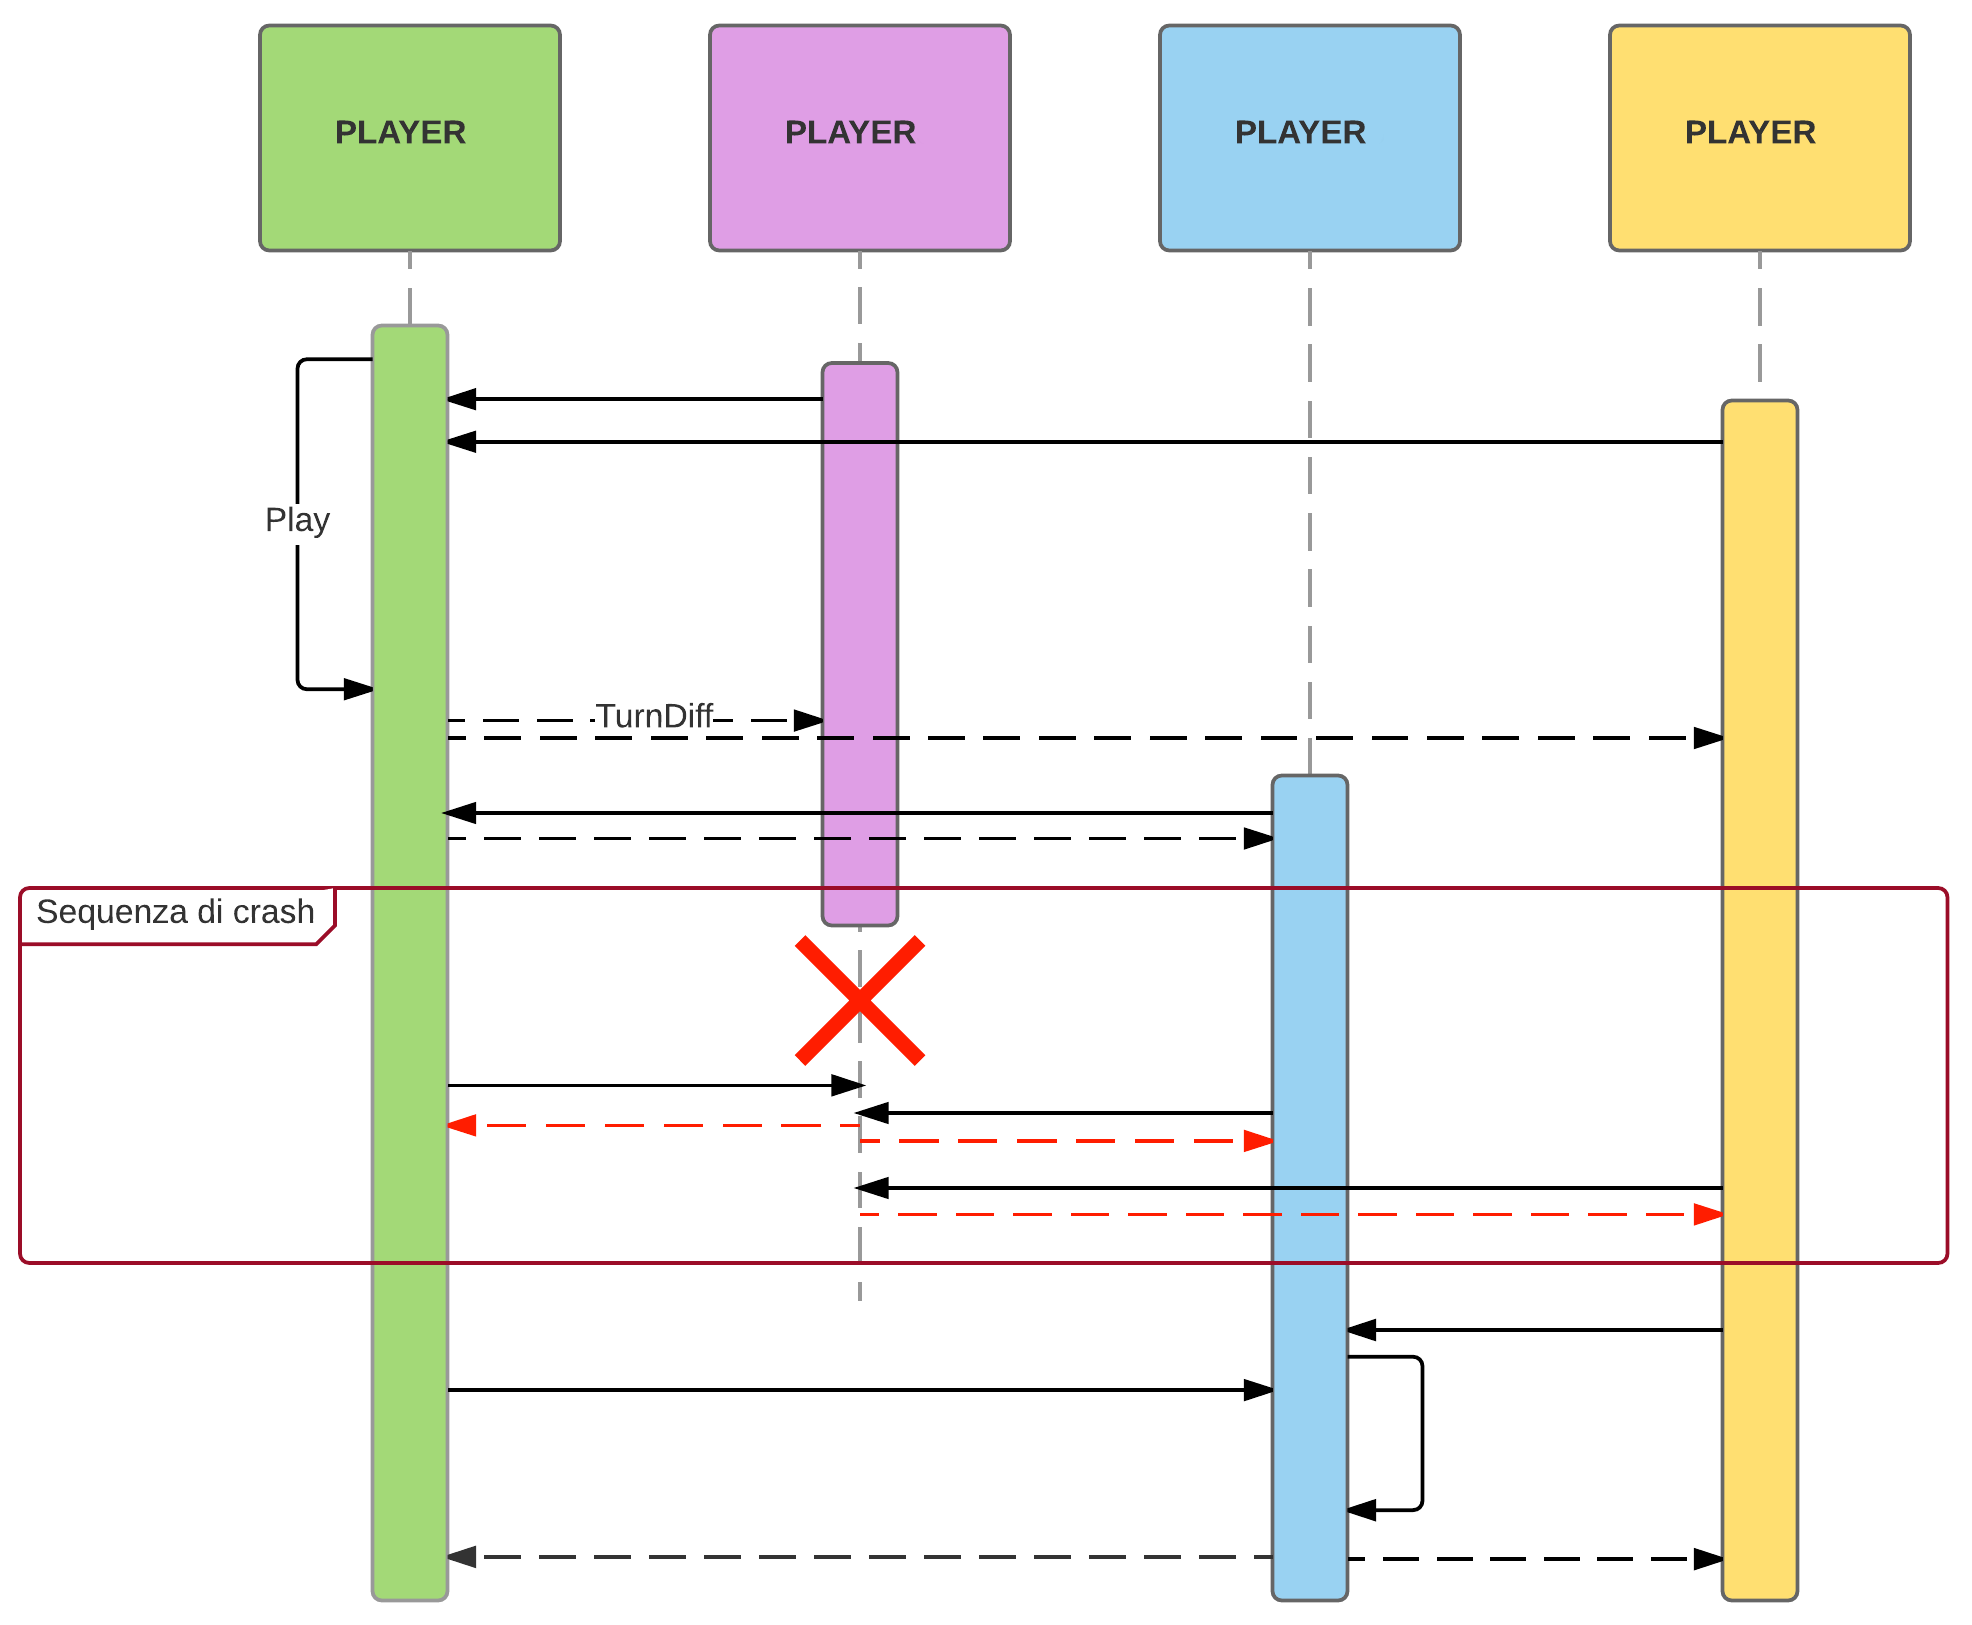
\includegraphics[width=\textwidth]{img/seq_diagram_play.png}
	\caption{Comunicazione in una partita d'esempio a 4 giocatori}
	\label{img:sequence}
\end{figure}

\subsubsection{Gestione della critical section}
	Il modello presenta una critical section ad ogni interrogazione di un leader
	(ogni nodo interrogante dovra' aspettare l'effettivo turno
	di gioco del leader), questa critical section e' implementata come un
	\textbf{Lock} a barriera utilizzando la classe \textbf{ReentrantLock}.\\
	Ogni nodo verra' bloccato fino all'avvenuto piazzamento della tessera e
	alla relativa creazione della struttura \textbf{TurnDiff}.\\
	Questo modello di critical section locale non invalida il meccanismo di
	tolleranza ai guasti poiche' se il processo leader subisce un
	\textbf{crash}, i vari richiedenti verranno liberati dalla critical
	section e gli verra' segnalato dal sistema di comunicazione il guasto.

\begin{figure}[H]
	\centering
	\includegraphics[width=\textwidth]{img/controllerClassDiagram.png}
	\caption{UML: Controller}
	\label{img:controller}
\end{figure}

